\section{Benchmark}

\begin{figure*}[!h]
\centering
\subfloat[Pluto]{\includegraphics[width=1.6in]{pluto-flappy-bird} \label{fig:pluto-flappy-bird}}
\hfil \subfloat[Unity]{\includegraphics[width=1.6in]{unity-flappy-bird} \label{fig:unity-flappy-bird}} \caption{Flappy Bird developed using Pluto and Unity} \label{fig:flappy-bird}
\end{figure*}

In this section, a benchmark between two engines will be shown, one engine will be using the techniques described in the sections below, the engine described in section \ref{sec:pluto} and the other one is the Unity, I'm choosing the Unity because I already have almost a decade of experience in it. For the benchmark, two games were developed using the engines, the game is a copy of Flappy Bird\footnote{"...Flappy Bird, developed by Gears Studio the concept is a simple, you have to tap a bird to make it fly and try to maneuver it through different obstacles the further you reach the higher your score will be being each obstacle 1 point."\cite{FlappyBird}} as shown in figure  \ref{fig:flappy-bird}. No specific optimizations were done for the chosen game but for the Unity the game will be compiled using both Mono\footnote{"Mono is an open source implementation of Microsoft's .NET Framework based on the ECMA standards for C\# and the Common Language Runtime."\cite{Mono}} and IL2CPP\footnote{"IL2CPP (Intermediate Language To C++) is a Unity-developed scripting backend which you can use as an alternative to Mono when building projects for various platforms. When building a project using IL2CPP, Unity converts IL code from scripts and assemblies to C++, before creating a native binary file (.exe, apk, .xap, for example) for your chosen platform. Some of the uses for IL2CPP include increasing the performance, security, and platform compatibility of your Unity projects."\cite{IL2CPP}} as scripting backend. All tests were run in the same environment, an Alienware 15 R3, Windows 10 64-bit, Intel i5-7300HQ CPU @ 2.5GHz, 32GB 2400MHz RAM, GTX 1060 6GB GPU and 500GB Samsung SSD 960 Evo. As shown in Mishra and Shrawankar's paper, this article will take benchmarks on CPU utilization, GPU utilization, frames per second and memory utilization\cite{ComparisonBetweenFamousGameEnginesAndEminentGames} as well the application load time and size in the disk.

\subsection{Development}
The development process is also an important thing to measure, since the implementation of the engine took more than half a year to reach this stable state and an additional week to develop the game, it was entirely developed in the source code without any visual editor tool to help the development. On the other hand, Unity is already available in the market and has an awesome visual editor to build games. With the Unity built-in tools were possible to develop the same game in almost four hours. So since unity already holds a bunch of features to help the game development, they won this one.
\subsection{Performance}
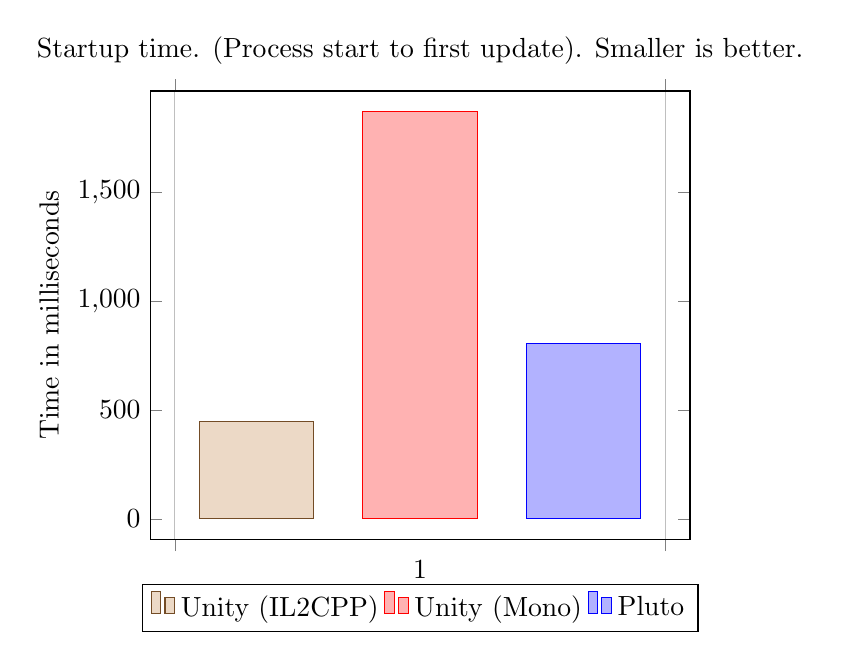
\begin{tikzpicture}
\begin{axis}[
    title={Startup time. (Process start to first update). Smaller is better.},
    reverse legend,
	x tick label style={
		/pgf/number format/1000 sep=},
	ylabel=Time in milliseconds,
	enlargelimits=0.05,
	legend style={at={(0.5,-0.1)},
	anchor=north,legend columns=-1},
	ybar interval=0.7,
]
\addplot 
	coordinates {(1,805) (0,0)};
\addplot 
	coordinates {(1,1870) (0,0)};
\addplot 
	coordinates {(1,445) (0,0)};
\legend{Pluto,Unity (Mono), Unity (IL2CPP)}
\end{axis}
\end{tikzpicture}
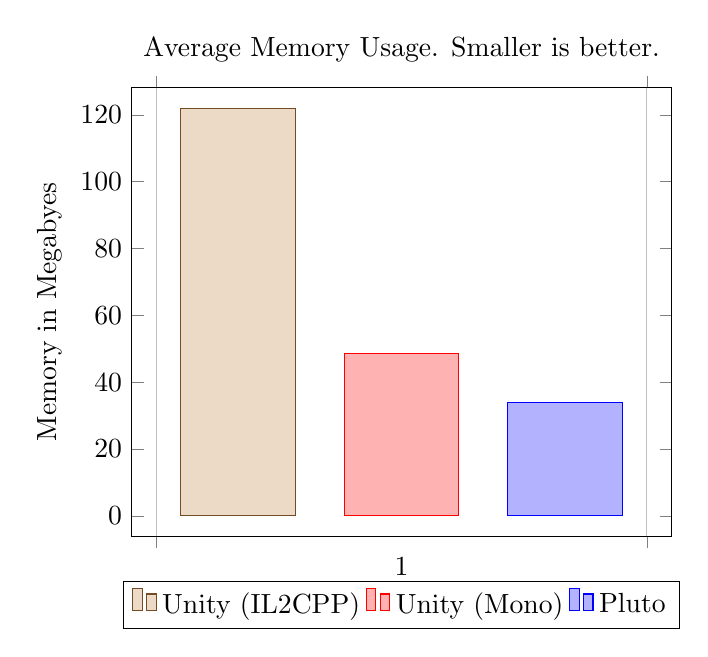
\begin{tikzpicture}
\begin{axis}[
    title={Average Memory Usage. Smaller is better.},
    reverse legend,
	x tick label style={
		/pgf/number format/1000 sep=},
	ylabel=Memory in Megabyes,
	enlargelimits=0.05,
	legend style={at={(0.5,-0.1)},
	anchor=north,legend columns=-1},
	ybar interval=0.7,
]
\addplot 
	coordinates {(1,34) (0,0)};
\addplot 
	coordinates {(1,48.5) (0,0)};
\addplot 
	coordinates {(1,122) (0,0)};
\legend{Pluto,Unity (Mono), Unity (IL2CPP)}
\end{axis}
\end{tikzpicture}
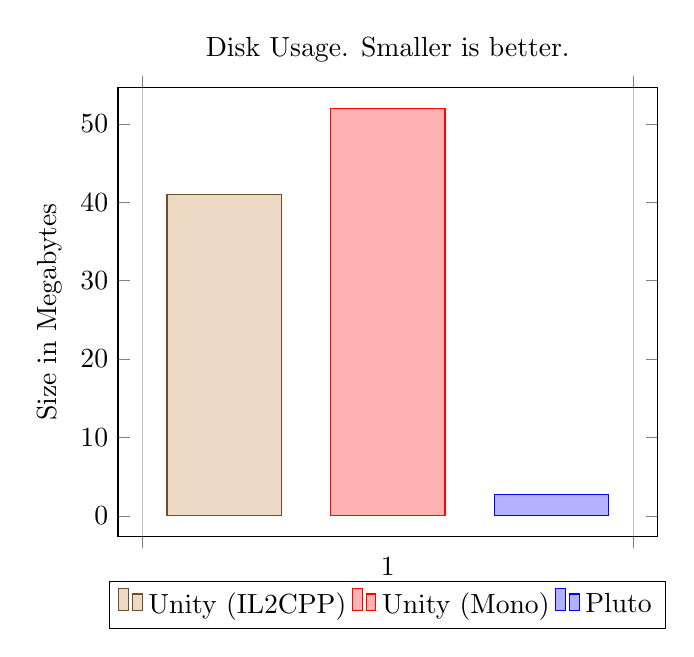
\begin{tikzpicture}
\begin{axis}[
    title={Disk Usage. Smaller is better.},
    reverse legend,
	x tick label style={
		/pgf/number format/1000 sep=},
	ylabel=Size in Megabytes,
	enlargelimits=0.05,
	legend style={at={(0.5,-0.1)},
	anchor=north,legend columns=-1},
	ybar interval=0.7,
]
\addplot 
	coordinates {(1,2.67) (0,0)};
\addplot 
	coordinates {(1,52) (0,0)};
\addplot 
	coordinates {(1,41) (0,0)};
\legend{Pluto,Unity (Mono), Unity (IL2CPP)}
\end{axis}
\end{tikzpicture}
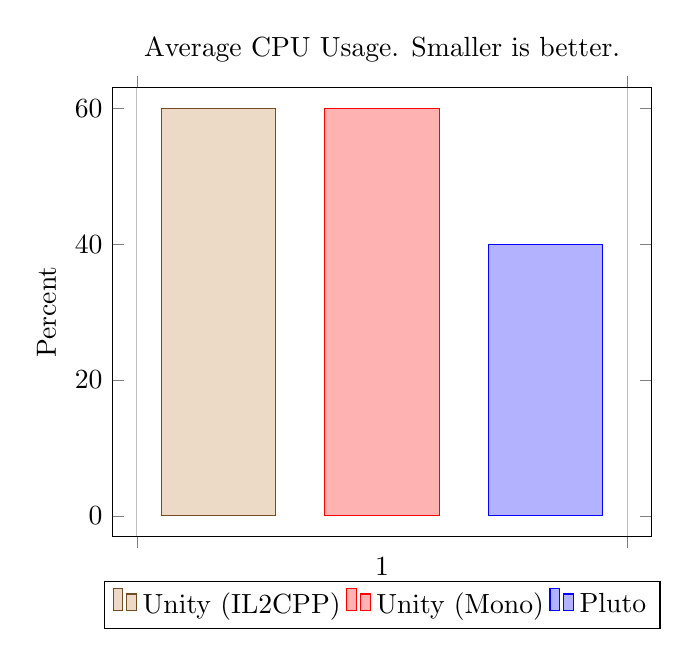
\begin{tikzpicture}
\begin{axis}[
    title={Average CPU Usage. Smaller is better.},
    reverse legend,
	x tick label style={
		/pgf/number format/1000 sep=},
	ylabel=Percent,
	enlargelimits=0.05,
	legend style={at={(0.5,-0.1)},
	anchor=north,legend columns=-1},
	ybar interval=0.7,
]
\addplot 
	coordinates {(1,40) (0,0)};
\addplot 
	coordinates {(1,60) (0,0)};
\addplot
	coordinates {(1,60) (0,0)};
\legend{Pluto,Unity (Mono), Unity (IL2CPP)}
\end{axis}
\end{tikzpicture}
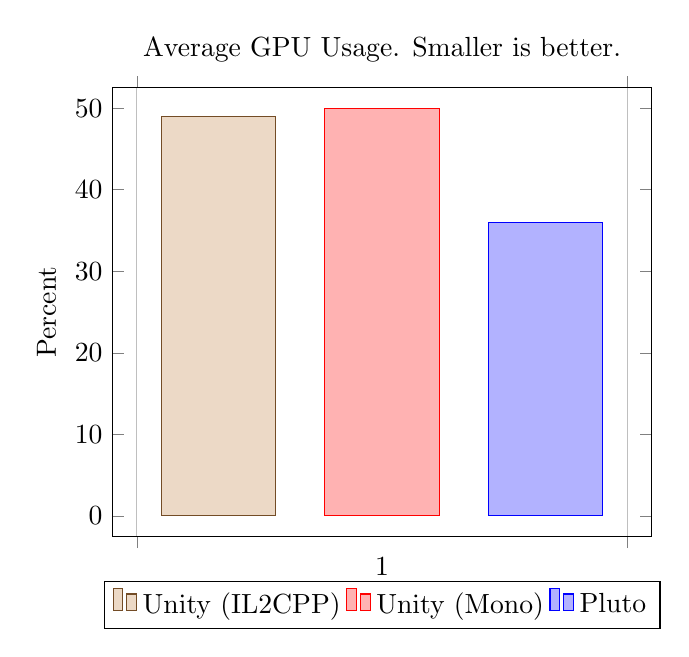
\begin{tikzpicture}
\begin{axis}[
    title={Average GPU Usage. Smaller is better.},
    reverse legend,
	x tick label style={
		/pgf/number format/1000 sep=},
	ylabel=Percent,
	enlargelimits=0.05,
	legend style={at={(0.5,-0.1)},
	anchor=north,legend columns=-1},
	ybar interval=0.7,
]
\addplot 
	coordinates {(1,36) (0,0)};
\addplot 
	coordinates {(1,50) (0,0)};
\addplot 
	coordinates {(1,49) (0,0)};
\legend{Pluto,Unity (Mono), Unity (IL2CPP)}
\end{axis}
\end{tikzpicture}
\begin{tikzpicture}[step y=500]
\begin{axis}[
    title={Average Frames per Second. Higher is better.},
    reverse legend,
	x tick label style={
		/pgf/number format/1000 sep=},
	ylabel=FPS,
	enlargelimits=0.05,
	legend style={at={(0.5,-0.1)},
	anchor=north,legend columns=-1},
	ybar interval=0.7,
]
\addplot 
	coordinates {(1,2632) (0,0)};
\addplot 
	coordinates {(1,2455) (0,0)};
\addplot
	coordinates {(1,3024) (0,0)};
\legend{Pluto,Unity (Mono), Unity (IL2CPP)}
\end{axis}
\end{tikzpicture}